\documentclass[openany,12pt,a4paper]{report}
\usepackage{subfiles}
\usepackage[numberedsection]{glossaries}
\usepackage[]{graphicx}
\usepackage{float}
\usepackage{multirow}
\graphicspath{{./img/}{./../img/}}
\usepackage{../StileDoc}
\title{Manuale Utente}
\author{}

%Ultima versione documento
\newcommand{\versione}{1.0.0}

% Stile per il glossario
\newglossarystyle{glossaryStyle}{
	\setglossarystyle{altlistgroup}
	\renewcommand*{\glsgroupheading}[1]{
		% Tolgo la numerazione per l'indice
		\setcounter{secnumdepth}{0}
		\section{##1}
		\vspace*{-\baselineskip}
		% Solo per fare un po' di spazio tra la lettera e le voci
		\item\makebox[\linewidth]{\hspace*{2cm}}
	}
}

\glsaddall

\makeglossaries

%Term definitions
\newglossaryentry{Speect}{name=Speect, description={Libreria di Text-To-Speech di riferimento per il progetto DeSpeect}}
\newglossaryentry{GCC}{name=GCC, description={Compilatore C++ di riferimento per il progetto DeSpeect}}
\newglossaryentry{GitHub}{name=GitHub, description={Servizio di versionamento per progetti software}}
\newglossaryentry{Qt}{name=Qt, description={Libreria multipiattaforma per lo sviluppo di programmi con interfaccia grafica tramite l'uso di widget}}
\newglossaryentry{utterance}{name={Utterance}, description={La più piccola unità del discorso, una parte di esso che inizia e termina con una pausa chiara}}
\newglossaryentry{relation}{name={Relation}, description={Rappresenta una struttura come una parola, sillaba, fonema o anche un obiettivo di durata e gli item sono il contenuto di questa struttura.}}
\newglossaryentry{framework}{name={Framework}, description={Piattaforma che funge da strato intermedio tra un sistema operativo e il software che lo utilizza.}}
\newglossaryentry{issue}{name={Issue}, description={Unità di lavoro per realizzare un miglioramento in un sistema. Un issue potrebbe essere un bug, una funzionalità richiesta, attività, documentazione mancante e così via.}}
\newglossaryentry{Curl}{name={Curl}, description={Curl è un tool da linea di comando o script utilizzato per trasferire dati.}}
\newglossaryentry{Swig}{name={Swig}, description={SWIG è un tool per lo sviluppo software che consente di collegare programmi scritti in C e C++ con una grande varietà di linguaggi ad alto livello}}
\newglossaryentry{label}{name={name},description={description}}
\newglossaryentry{libxml2-dev}{name={libxml2-dev}, description={File di sviluppo in proprio di programmi che utilizzano la libreria Gnome XML}}
\newglossaryentry{python-dev}{name={python-dev}, description={è una collezione di tool per sviluppatori Python presentata come alternativa a ciò che viene offerto dalla libreria standard.}}
\newglossaryentry{HRG}{name={HRG}, description={Heterogeneous Relation Graph: struttura dati per memorizzare le informazioni di un utterance in Speect.}}
\newglossaryentry{JSon}{name={JSon}, description={Formato di file leggero adatto allo scambio dati, autodescrittivo e indipendente dalla lingua usata.}}
\newglossaryentry{voice}{name={voice},description={Una voice definisce gli utterance type che possono essere utilizzati per la sintesi con la voce specifica}}
\newglossaryentry{file Voice}{name={File Voice}, description={File di inizializzazione di Speect}, nonumberlist }

\begin{document}
	\makeatletter
	\begin{titlepage}
		\setlength{\headsep}{0pt}  
		\begin{center}
			
\includegraphics[width=0.5\linewidth]{img/logo.png}\\[1em]
			{\huge \bfseries  \@title }\\[10ex]
			\textbf{\Large Informazioni Documento} \\[2em]
			\bgroup
			\def\arraystretch{1.5}
			\begin{tabular}{l|l}
				\textbf{Versione} & \versione{} \\
				\textbf{Redattori} & Marco Focchiatti, Giulio Rossetti, \\
				& Kevin Silvestri, Matteo Rizzo \\
				\textbf{Verificatori} & Manfredi Smaniotto, Samuele Modena \\
				\textbf{Distribuzione} & Prof. Tullio Vardanega \\
				& Prof. Riccardo Cardin \\
				& Mivoq S.R.L. \\
				& Gruppo Graphite \\
				\textbf{Uso} & Esterno \\
				\textbf{Recapito} & graphite.swe@gmail.com \\
			\end{tabular}
			\egroup
		\end{center}
	\end{titlepage}
	\makeatother
	
	\thispagestyle{empty}
	\newpage
	
	%REGISTRO DELLE MODIFICHE
	
	\chapter*{Registro delle modifiche}
	\setlength\LTleft{-22mm}
	\begin{longtable}{|p{20mm}|p{20mm}|p{40mm}|p{30mm}|p{50mm}|}
		\hline
		\textbf{Versione} & \textbf{Data} & \textbf{Autore} & \textbf{Ruolo} & \textbf{Descrizione} \\
		
		\hline 0.2.0 & 2018-04-12 & Samuele Modena & Verificatore & Verifica §5 e §A\\
		\hline 0.1.2 & 2018-04-11 & Matteo Rizzo & Amministratore & Stesura §A \\	
		\hline 0.1.1 & 2018-04-11 & Kevin Silvestri & Progettista & Stesura §5 \\
		\hline 0.1.0 & 2018-04-10 & Manfredi Smaniotto & Verificatore & Verifica da §1 a §4 \\
		\hline 0.0.5 & 2018-04-09 & Marco Focchiatti & Programmatore & Stesura §4 \\	
		\hline 0.0.4 & 2018-04-09 & Giulio Rossetti & Programmatore & Stesura §3 \\
		\hline 0.0.3 & 2018-04-08 & Kevin Silvestri & Programmatore & Stesura §2 \\
		\hline 0.0.2 & 2018-04-08 & Matteo Rizzo & Amministratore & Stesura §1 \\
		\hline 0.0.1 & 2018-04-08 & Matteo Rizzo & Amministratore & Creata struttura documento \\
		\hline
		
	\end{longtable}
	
	% INDICE
	\tableofcontents
	
	% INTRODUZIONE
	
	\chapter{Introduzione}
	
	\section{Scopo del documento}
	
	Il documento ha la finalità di illustrare, a coloro che volessero interfacciarsi con l’applicazione
	\textit{"DeSpeect: un'interfaccia grafica per Speect"}, i requisiti necessari per poterlo utilizzare e le modalità di installazione e di utilizzo. 
	Nonostante la versione attuale rappresenti una prima bozza del documento, una volta concluso esso rappresenterà sia una guida che un riferimento completo per l’utilizzo del prodotto da parte di un utente.
	
	\section{Scopo del prodotto}
	
	Lo scopo del progetto è la realizzazione di un’interfaccia grafica per \glossario{Speect}{Speect} [Meraka Institute(2008-2013)], una libreria per la creazione di sistemi di sintesi vocale, che agevoli l’ispezione del suo stato interno durante il funzionamento e la scrittura di test per le sue funzionalità.
	
	\section{Informazioni utili}
	
	La stesura di questo documento assume come utente target del prodotto un programmatore esperto nell'utilizzo di \textit{Speect}. \\
	\noindent Per completezza, viene riportato in appendice §A un glossario comprensivo di termini tecnici o riguardanti particolari funzionalità di \textit{DeSpeect}. Per identificare i termini presenti nel glossario, la loro prima occorrenza all’interno del documento è riportata in corsivo e marcata con una G al pedice. 
	
	%quando caricheremo su github in una repository apposita il manuale sviluppatore
	\begin{comment}
	\\ \noindent Per i manutentori del prodotto o per chi fosse interessato alla sua integrazione/incremento, può invece consultare il manuale sviluppatore reperibile all'indirizzo: \url{...}
	\end{comment}

	\newpage
	
	\section{Riferimenti informativi}

	\begin{itemize}
		\item \textbf{Documentazione Speect:} \\
		\url{http://speect.sourceforge.net/contents.html};
		\subitem Documentazione ufficiale della libreria di \textit{Text-To-Speech} di riferimento per il progetto.
		
		\item \textbf{Documentazione Qt:} \\
		\url{http://doc.qt.io/};
		\subitem Documentazione ufficiale del \glossario{framework}{framework} utilizzato per lo sviluppo dell'interfaccia grafica.
		
		\item \textbf{Documentazione CMake:} \\
		\url{https://cmake.org/documentation/}.
		\subitem Documentazione ufficiale del framework utilizzato per la build del prodotto. 
	\end{itemize}

	\chapter{Requisiti di sistema}
	
	\section{Requisiti hardware}
	
	L'installazione ed esecuzione del software DeSpeect richiede una macchina con i seguenti requisiti:
	\begin{center}
		\begin{longtable}{| p{40mm} | p{60mm} | p{60mm} |}
			\hline
			\textbf{Hardware} & \textbf{Requisiti minimi} & \textbf{Requisiti consigliati} \\
			\hline CPU & 2 GHz dual core x86 & 3GHz quad core x64 \\
			\hline RAM & 4 GB & 8GB \\
			\hline Spazio libero su disco & 256MB & 1GB \\
			\hline  \multirow{3}{*}{GPU}
			& accelerazione video 3D & accelerazione video 3D \\ 
			& risoluzione 1280x1024 & risoluzione 1920x1080 \\
			& 256 MiB di memoria & 512 MiB di memoria \\
			\hline
		\end{longtable}
	\end{center}
	\section{Requisiti software}
	
	L'installazione ed esecuzione del software DeSpeect richiede i seguenti programmi preinstallati:
	
	\begin{itemize}
		\item Sistema operativo Unix / Unix-like (il software è stato testato solo per piattaforma Ubuntu 16.04 LTS)
		\subitem \url{https://www.ubuntu.com/download/desktop}
		\item CMake (versione minima 2.8)
		\subitem \url{https://cmake.org/download/}
		\item Compilatore ANSI C/ISO C90 \glossario{GCC}{GCC} (versione minima 5.0)
		\subitem \url{https://gcc.gnu.org/install/binaries.html}
		\item \glossario{Qt}{Qt} 5.9.0
		\subitem \url{https://www.qt.io/download}
		\item Git
		\subitem \url{https://git-scm.com/} 
		\item Curl 
		\subitem \url{https://curl.haxx.se/}
		\item Swig 
		\subitem \url{http://www.swig.org/}
		\item libxml2-dev
		\subitem \url{https://packages.debian.org/stretch/libxml2-dev} 
		\item python-dev
		\subitem \url{https://pypi.python.org/pypi/dev/0.4.0}
	\end{itemize}
	
	 
	\chapter{Installazione e configurazione} 
	
	DeSpeect è reperibile su GitHub al seguente link:
	\begin{center}
		\url{https://github.com/graphiteSWE/DeSpeect}
	\end{center}
	
	\noindent Una volta soddisfatti i prerequisiti descritti in §2 "Requisiti di sistema" di questo documento, per installare ed eseguire il software è necessario seguire la seguente procedura:
	\begin{enumerate}
		\item Clonare o scaricare il repository sulla propria macchina;
		\item Entrare nella cartella scaricata ed eseguire lo script \verb|build.sh| presente al suo interno. Tale script installerà Speect ed effettuerà una build del progetto all'interno nella directory \verb|DeSpeect/build/|.
		\item Per eseguire DeSpeect, entrare nella directory \verb|DeSpeect/build/bin/| ed eseguire il comando \verb|./main|.
	\end{enumerate}
	
	\chapter{Guida all'utilizzo}
	Viene di seguito illustrata la guida all'utilizzo del software DeSpeect. \\
	Si fa notare che i termini evidenziati in \textit{corsivo} corrispondono a pulsanti specifici presenti all'interno dell'applicazione.
	
	\section{Struttura dell'interfaccia grafica}
	
	\begin{figure}[H]
		
		\centering
		
		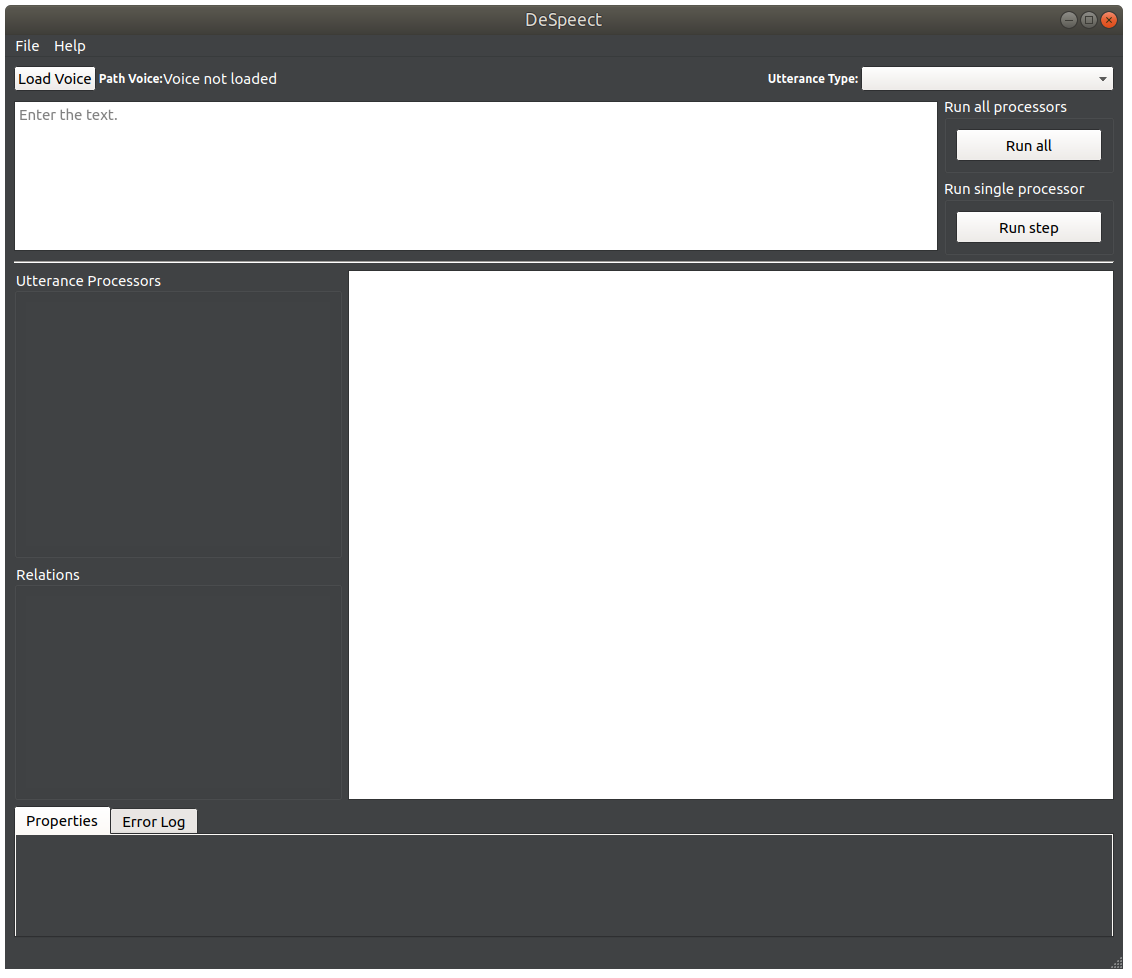
\includegraphics[scale=0.3]{./img/main-window}
		
		\caption{Interfaccia grafica - Schermata iniziale}
	
	\end{figure}

	All'avvio dell'applicazione viene presentata la schermata riportata in Figura 4.1. L'interfaccia grafica è costituita dalle componenti illustrate nelle sezioni seguenti.
 	
 	\subsection{Menù dell'applicazione}
 	
 	\begin{figure}[H]
 		
 		\centering
 		
 		
\includegraphics{./img/menu}
 		
 		\caption{Menù dell'applicazione - Visione generale}
 		
 	\end{figure}
 
 	Menù situato nella parte superiore della schermata. Tramite il menù \textit{File} è possibile interagire con alcune funzionalità offerte dal sistema, mentre tramite il menù \textit{Help} è possibile visualizzare manuale utente e licenza del prodotto (vedi Figura 4.2). Il menù è sempre disponibile in qualunque posizione all'interno dell'applicazione e al suo interno è possibile selezionare le seguenti voci:
 	
 	\newpage
 	
 	\subsubsection{File} 
 		\begin{itemize}
 			\item \textbf{Load Voice JSon}: carica il \glossario{file Voice}{file Voice} \glossario{JSon}{JSon};
 			\item \textbf{Save Audio file}: salva il file audio prodotto in seguito all'esecuzione di \textit{Speect};
 			\item \textbf{Search path}: cerca un nodo inserendo come input un percorso specifico (es. Words.parent.n);
 			\item \textbf{Exit}: chiude l'interfaccia \textit{DeSpeect}.
 		\end{itemize}
 		
 		\begin{figure}[H]
 			
 			\centering
 			
 			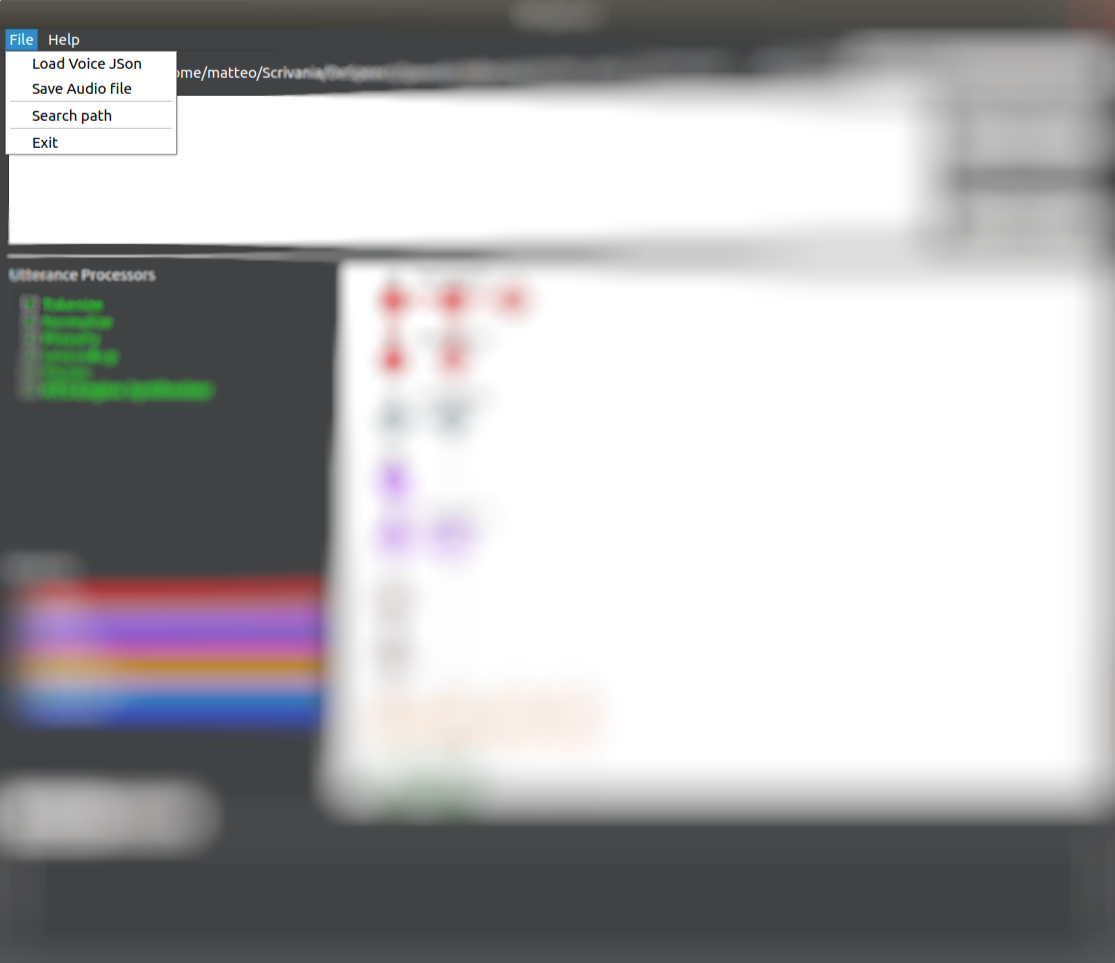
\includegraphics[scale=0.3]{./img/file}
 			
 			\caption{Menù dell'applicazione - Sezione "File"}
 			
 		\end{figure}
 	
 	\newpage
 	
 	\subsubsection{Help}
 		\begin{itemize}
 			\item \textbf{Manual}: apre il manuale utente;
 			\item \textbf{Licence}: visualizza la licenza di \textit{DeSpeect}.
 		\end{itemize}
 		\begin{figure}[H]
 			
 			\centering
 			
 			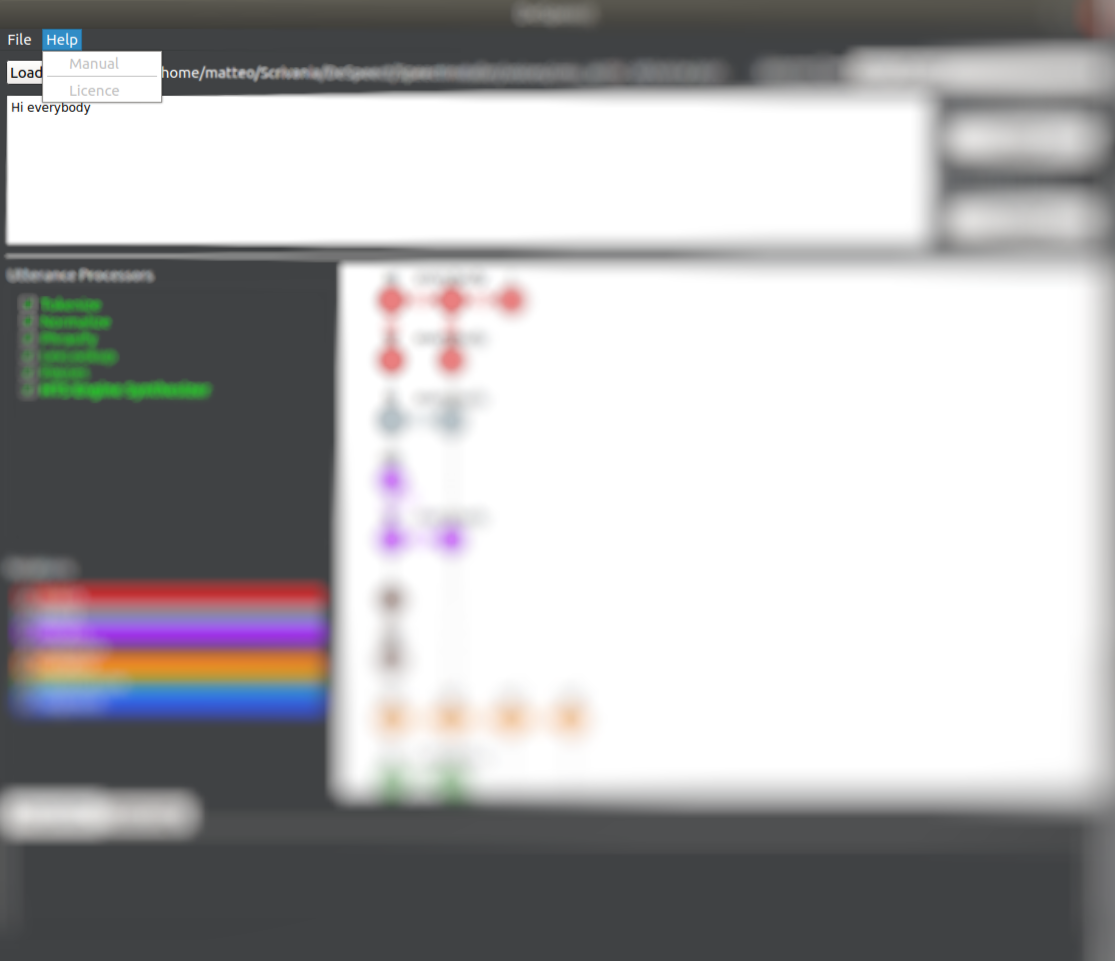
\includegraphics[scale=0.3]{./img/help}
 			
 			\caption{Menù dell'applicazione - Sezione "Help"}
 			
 		\end{figure}
 	
 	\newpage
 	
 	\subsection{Pannello di configurazione}
 	Situato nella parte superiore della schermata sotto il menù citato al punto precedente. Qui è possibile caricare un file Voice (tramite pulsante \textit{Load Voice}), inserire input testuale (tramite area di testo dedicata), selezionare l'\glossario{utterance}{utterance} type e avviare l'esecuzione di \textit{Speect} eseguendo singolarmente ogni utterance processor (pulsante \textit{Run step}) o tutti assieme in sequenza (pulsante \textit{Run all}).
 		\begin{figure}[H]
 			
 			\centering
 			
 			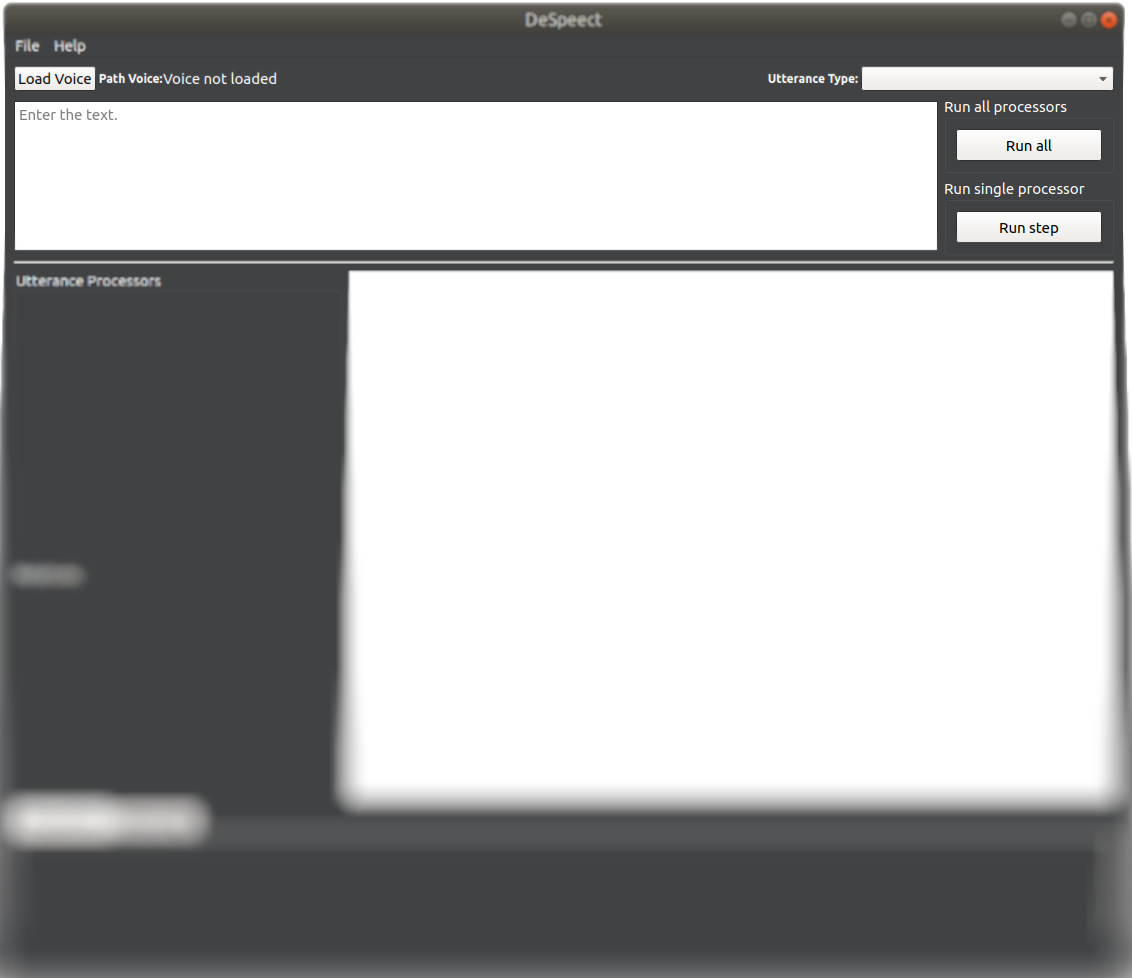
\includegraphics[width=\textwidth]{./img/config-panel}
 			
 			\caption{Interfaccia grafica - Pannello di configurazione}
 			
 		\end{figure}
 	
 	\newpage
 	
 	\subsection{Pannello degli utterance processor}
 	Situato sulla sinistra, sotto al pannello di configurazione. Qui è presente una lista degli utterance processor relativi alla \glossario{voice}{voice} caricata e all'utterance type selezionata, a ognuno dei quali è assegnata una checkbox. Spuntando le checkbox l'utente seleziona gli utterance processor che desidera eseguire per un dato input tramite i pulsanti dedicati presenti nel pannello di configurazione (pulsanti \textit{Run all} e \textit{Run step}). Avviata l'esecuzione, i processor eseguiti verranno evidenziati dal colore verde, mentre quello corrente è riportato in grassetto (vedi Figura 4.4);
 		\begin{figure}[H]
 			
 			\centering
 			
 				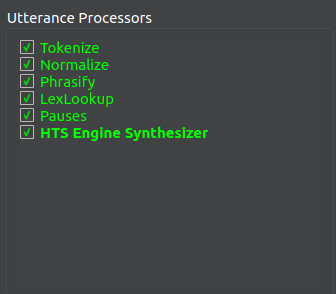
\includegraphics[width=.4\textwidth]{./img/utterance-processors}
 			
 			\caption{Interfaccia grafica - Pannello degli utterance processors}
 			
 		\end{figure}
 		
 	\subsection{Pannello delle relations}
 	Situato sulla sinistra, sotto al pannello degli utterance processor. Qui è possibile selezionare quali \glossario{relation}{relation} visualizzare nel grafo. Di default, il grafo mostra ogni relation disponibile, rimuovendo la spunta dalla checkbox della relation desiderata le componenti del grafo relative vengono rimosse dalla visualizzazione (vedi Figura 4.5);
 		\begin{figure}[H]
 			
 			\centering
 			
 				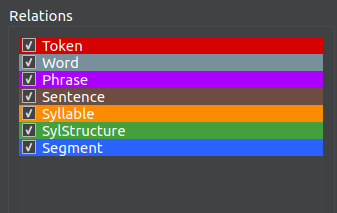
\includegraphics[width=.4\textwidth]{./img/relations}
 			
 			\caption{Interfaccia grafica - Pannello delle Relations}
 			
 		\end{figure}
 	
 	\subsection{Area del grafo}
 	Situata sulla destra, sotto al pannello di configurazione. Qui viene visualizzato il grafo relativo ad una data voice, input testuale e configurazione di utterance processor. I nodi sono selezionabili (nel cui caso, le informazioni relative al nodo vengono visualizzate nell'apposita barra approfondita al punto seguente) e spostabili (vedi Figura 4.6);
 		\begin{figure}[H]
 			
 			\centering
 			
 				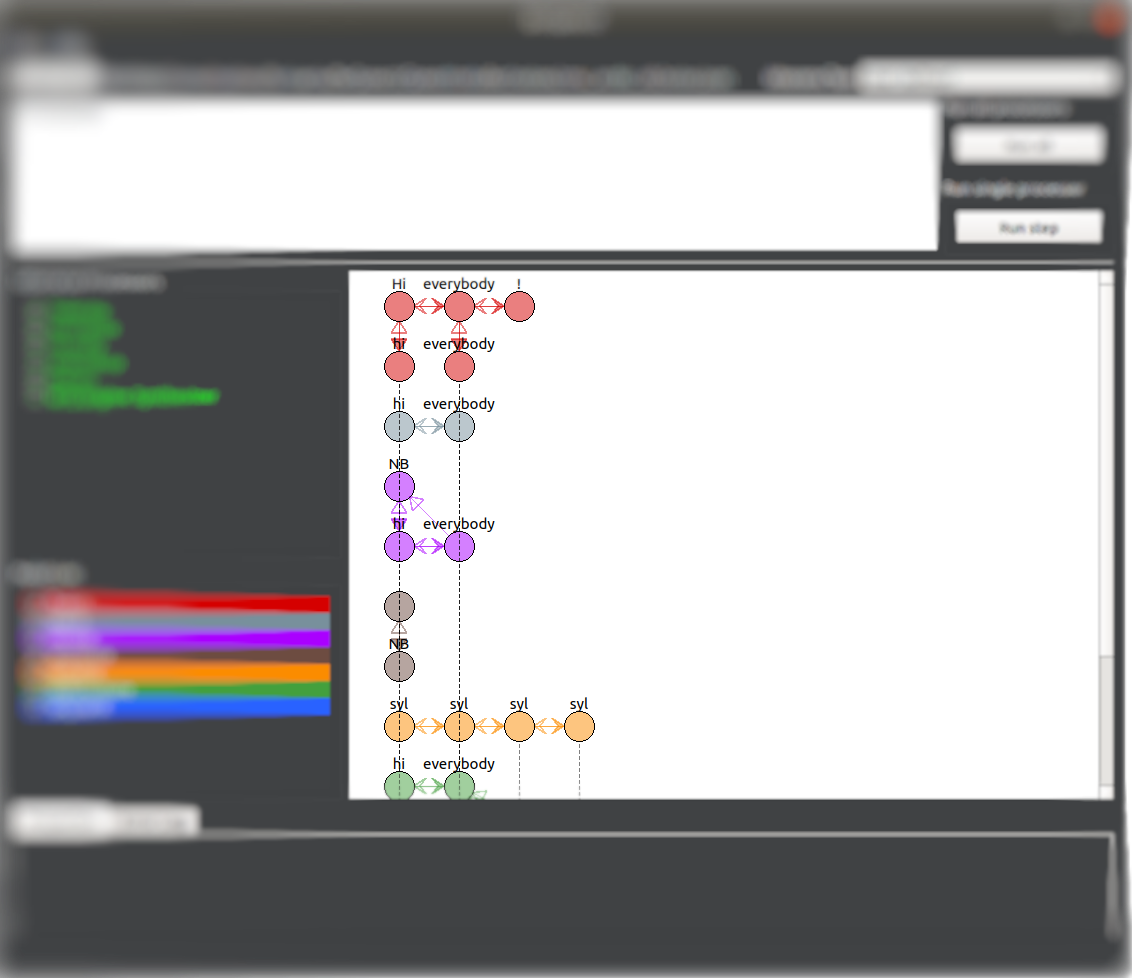
\includegraphics[scale=0.3]{./img/graph-area}
 			
 			\caption{Interfaccia grafica - Area del grafo}
 			
 		\end{figure}
 	
 	\subsection{Proprietà del nodo}
 	Situato nella parte inferiore dell'interfaccia. Qui vengono visualizzate le informazioni specifiche relative al nodo selezionato (vedi Figura 4.7).
 		\begin{figure}[H]
 			
 			\centering
 			
 				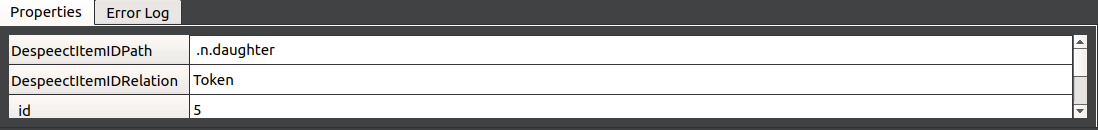
\includegraphics[width=\textwidth]{./img/node-properties}
 			
 			\caption{Interfaccia grafica - Proprietà del nodo}
 			
 		\end{figure}
	
	\section{Interagire con la voice}
	Questa sezione tratta dell'interazione con la voice (rappresentata da un file \verb|.json|), dal suo caricamento alla generazione dell'audio prodotto da \textit{Speect}.
	
	\subsection{Caricare la voice}
	Per caricare la voice è sufficiente cliccare il pulsante \textit{Load Voice}, situato nell'angolo in alto a sinistra del pannello di configurazione (vedi §4.1.2) o, in alternativa, cliccare sul menù \textit{File} e, successivamente, sulla voce \textit{Load Voice}.\\
	Una volta fatto ciò si aprirà il file browser del sistema operativo, che permetterà la ricerca di un file \verb|.json| corrispondente alla voice desiderata. Una volta reperito il file, sarà sufficiente aprirlo mediante file browser.\\
	A questo punto, se verrà visualizzato il percorso del file \verb|.json| subito dopo l'etichetta "Path Voice", vicino al pulsante di caricamento della voice, allora il caricamento della stessa avrà avuto successo.\\
	Nel caso in cui il caricamento del file abbia avuto esito negativo, è necessario ripetere la procedura assicurandosi si averla eseguita correttamente.
	
	\subsubsection*{Esempio}
	
	In questo esempio, si mostra come caricare una voice open source fornita con Speect. Sarà necessario attenersi alla seguente procedura:
	\begin{enumerate}
		\item cliccare il pulsante \textit{Load Voice} o su \textit{File} e successivamente  \textit{Load Voice}";
	\end{enumerate} 
	
	\subsection{Salvare l'audio relativo alla voice}
	Uno volta eseguito \textit{Speect}, per salvare l'audio è sufficiente cliccare sul pulsante \textit{File} del menù e selezionare la voce \textit{Save Audio file}.\\
	Fatto ciò, si aprirà una finestra di ricerca del file browser dove cercare la cartella in cui salvare il file. Una volta trovata basterà selezionarla, cliccandoci sopra o scrivere il nome del nuovo file nella barra di testo dedicata e confermare, con attenzione di riportare l'estensione \verb|.wav|.\\
	Il file audio prodotto avrà l'estensione \verb|.wav|.
	Questa operazione controllerà se è possibile salvare l'audio e come ogni altra operazione darà un report nella log di errore.
	
	\section{Visualizzare il grafo}
	Per visualizzare il grafo è necessario aver caricato una voice, inserito un input testuale ed eseguito \textit{Speect} tramite pulsante \textit{Run all} o \textit{Run step}.\\
	Se sono state compiute tali azioni, viene visualizzato il grafo nell'area dedicata (§4.1.5), nonché la lista delle relation (§4.1.4).
	Il grafo è composto da:
	\begin{itemize}
		\item \textbf{Nodi}: visualizzati tramite cerchi con relativo name, i nodi hanno colori diversi a seconda della relazione a cui appartengono (la lista delle relation funge da legenda);
		\item \textbf{Archi}: visualizzati tramite frecce direzionali che collegano due nodi, anche gli archi sono di colori diversi a seconda della relazione a cui fanno riferimento e sono differenziati in base alla tipologia:
		Inserire Immagine archi con descrizione	Inserire Immagine archi con descrizione	Inserire Immagine archi con descrizione	Inserire Immagine archi con descrizione	Inserire Immagine archi con descrizione	Inserire Immagine archi con descrizione	Inserire Immagine archi con descrizione	Inserire Immagine archi con descrizione	Inserire Immagine archi con descrizione	Inserire Immagine archi con descrizione	Inserire Immagine archi con descrizione	Inserire Immagine archi con descrizione	Inserire Immagine archi con descrizione	Inserire Immagine archi con descrizione	Inserire Immagine archi con descrizione	Inserire Immagine archi con descrizione	Inserire Immagine archi con descrizione	Inserire Immagine archi con descrizione	Inserire Immagine archi con descrizione	Inserire Immagine archi con descrizione	Inserire Immagine archi con descrizione	Inserire Immagine archi con descrizione	Inserire Immagine archi con descrizione
	\end{itemize}
	
	\subsection{Visualizzare il grafo step-by-step}
	Eseguendo \textit{Speect} tramite pulsante \textit{Run step}, è possibile eseguire un utterance processor alla volta e vederne il risultato sul grafo, che ad ogni step si aggiorna aggiungendo nuove relazioni.
	
	\subsection{Visualizzare l'intero grafo}
	Eseguendo \textit{Speect} tramite pulsante \textit{Run all} è possibile eseguire tutti gli utterance processor in una sola volta e vedere subito il grafo completo.
	
	\section{Interagire con il grafo}
	Questa sezione spiega come poter interagire col grafo spostando nodi e archi, rimuovendo nodi e archi relativi a determinate relation dalla visualizzazione.
	
	\subsection{Selezionare gli utterance processors}
	Nel pannello degli utterance processor (§4.1.3) è possibile interagire con i processor tramite le caselle di spunta a lato.\\
	Togliendo la spunta da un processor, esso non verrà eseguito da \textit{Speect}, e viceversa.
	
	\subsection{Interagire con le relations}
	Nel pannello delle relation è possibile interagire con esse tramite le caselle di spunta a lato.\\
	Togliendo la spunta da una relation, i relativi nodi verranno rimossi dalla visualizzazione del grafo, viceversa se si aggiunge la spunta, verranno aggiunti i relativi nodi al grafo.
	
	\subsection{Traslare elementi grafici}
	Questa sezione spiega come traslare gli elementi grafici che compongono il grafo, ovvero nodi e archi.
	
	\subsubsection{Traslare nodi}
	Per traslare un nodo è sufficiente cliccare su di esso tenendo premuto e, spostando il cursore, trascinarlo dove si desidera all'interno dell'area del grafo.
	Inoltre è possibile selezionare più nodi tenendo premuto CTRL durante la selezione
	
	\subsubsection{Traslare archi}
	Quando si trasla un nodo, gli archi che sono coinvolti direttamente con quel nodo si adatteranno alla nuova posizione del nodo.
	
	\chapter{Risoluzione dei problemi}
	
	\section{Errori in DeSpeect}
	Gli errori che si possono riscontrare utilizzando l’applicazione verrano stampati nella log di errore, nel caso l'errore sia dell'engine Speect il suo errore verrà riportato nel file ErrorLog.txt \textit{DeSpeect}.
	\subsection{Struttura dei codici di errore}
	Gli errori rispettano la seguente notazione:
	
	\begin{center}
		Operazione in esecuzione,Operation Status: stato di Speect in seguito all'operazione.
		Gli stati sono:
		\begin{itemize}
			\item {No error} Successo, nessun errore;
			\item {Failure} Una failure non specificata è avvenuta;
			\item {Memory allocation failed} Errore di allocazione di memoria;
			\item {Function argument(s) invalid} Errore negli argomenti della funzione;
			\item {Class/object method does not exist} Classe/Oggetto non esistono;
			\item {End of file/stream} Fine del file o dello stream raggiunta;
			\item {Warning, possible error} Attenzione possibile errore;
			\item {Error context continued} Errore il contesto continua;
			\item {Undefined error} Errore non definito.
		\end{itemize}
	 	Se l'operazione finisce in uno stato diverso da No error, nel file ErrorLog.txt verrà descritto in maniera più dettagliata.
	\end{center}
	
	\section{Problemi con il reperimento di Speect}	
	Il portale che ospita documentazione e download di \textit{Speect} può occasionalmente risultare offline per dei giorni.\\
	Si consiglia di scaricare in locale  tutto il materiale reperibile online così da tutelarsi nel caso il problema dovesse occorrere.
	
	\section{Segnalazione di bug}
	
	\textit{DeSpeect} potrebbe contenere bug o potrebbe essere desiderabile apportare modifiche e ampliamenti alle sue funzionalità. \\ È possibile segnalare malfunzionamenti o richieste di nuove funzionalità sotto forma di GitHub \glossario{issue}{issue} all’indirizzo:
	\begin{center}
		\url{https://github.com/graphiteSWE/DeSpeect}
	\end{center}
  oppure scrivendo direttamente all'indirizzo e-mail:
  \begin{center}
  	\url{graphite.swe@gmail.com}
  \end{center}
	
	\appendix
	
	\printglossary[style=glossaryStyle, nonumberlist]
	
\end{document}
